\documentclass{standalone}
\usepackage{tikz}
\usetikzlibrary{patterns, positioning}


\begin{document}
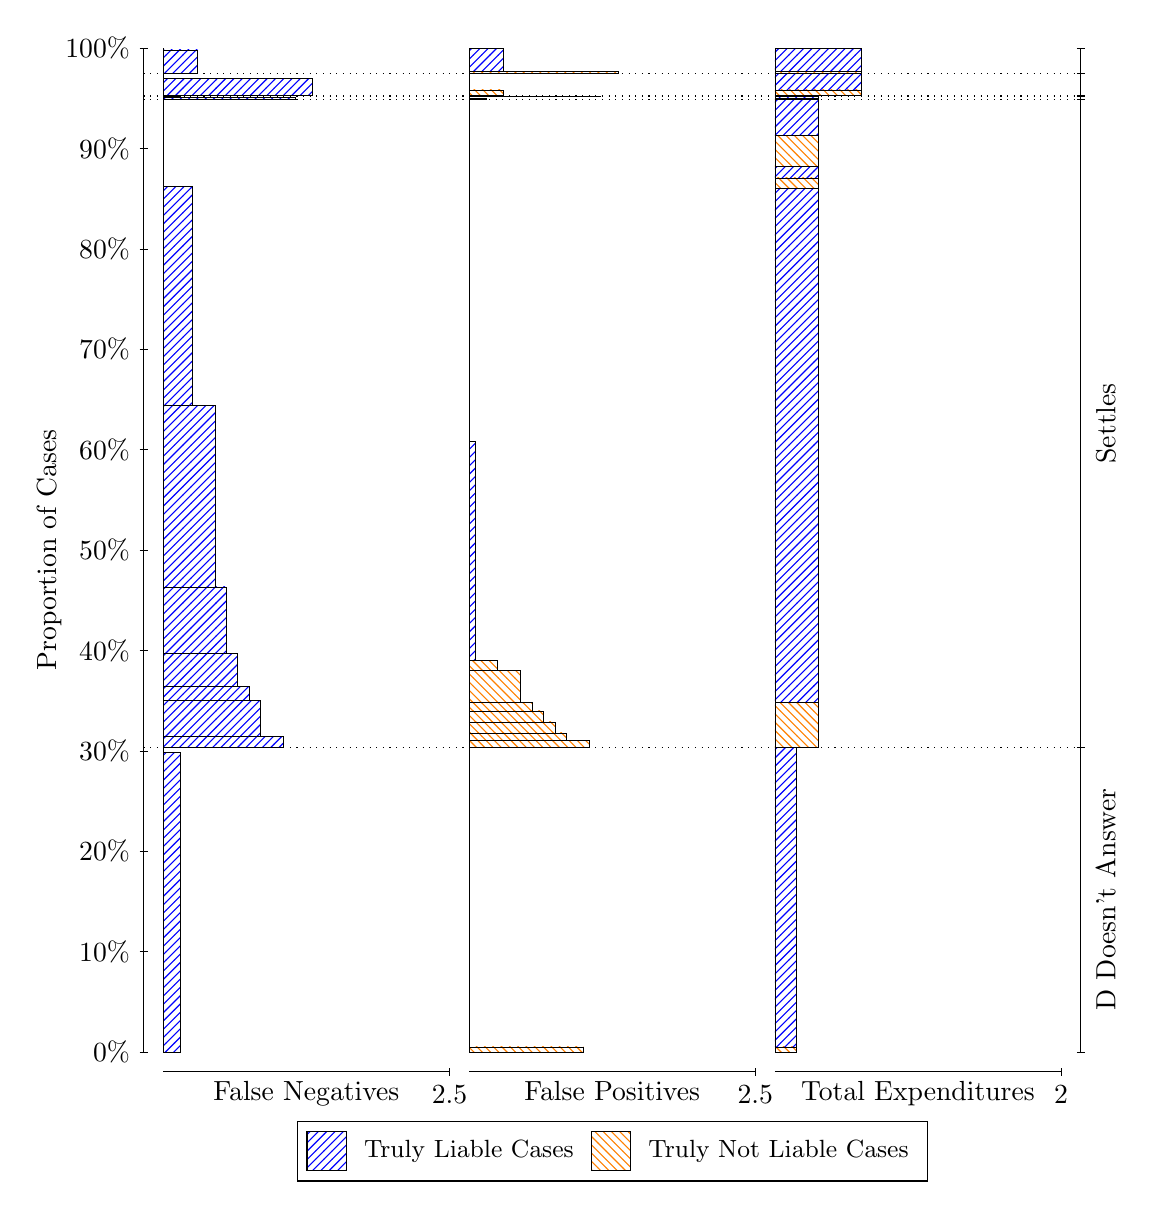
\begin{tikzpicture}
\draw[black, very thin] (1.5,1.75) -- (1.5,14.5);
\node[rotate=90, text=black, anchor=center] at (0.3, 8.125) {Proportion of Cases};
\draw[black, very thin] (1.45,1.75) -- (1.55,1.75);
\node[text=black, anchor=east] at (1.45, 1.75) {0\%};
\draw[black, very thin] (1.45,3.025) -- (1.55,3.025);
\node[text=black, anchor=east] at (1.45, 3.025) {10\%};
\draw[black, very thin] (1.45,4.3) -- (1.55,4.3);
\node[text=black, anchor=east] at (1.45, 4.3) {20\%};
\draw[black, very thin] (1.45,5.575) -- (1.55,5.575);
\node[text=black, anchor=east] at (1.45, 5.575) {30\%};
\draw[black, very thin] (1.45,6.85) -- (1.55,6.85);
\node[text=black, anchor=east] at (1.45, 6.85) {40\%};
\draw[black, very thin] (1.45,8.125) -- (1.55,8.125);
\node[text=black, anchor=east] at (1.45, 8.125) {50\%};
\draw[black, very thin] (1.45,9.4) -- (1.55,9.4);
\node[text=black, anchor=east] at (1.45, 9.4) {60\%};
\draw[black, very thin] (1.45,10.675) -- (1.55,10.675);
\node[text=black, anchor=east] at (1.45, 10.675) {70\%};
\draw[black, very thin] (1.45,11.95) -- (1.55,11.95);
\node[text=black, anchor=east] at (1.45, 11.95) {80\%};
\draw[black, very thin] (1.45,13.225) -- (1.55,13.225);
\node[text=black, anchor=east] at (1.45, 13.225) {90\%};
\draw[black, very thin] (1.45,14.5) -- (1.55,14.5);
\node[text=black, anchor=east] at (1.45, 14.5) {100\%};

\draw[black, very thin] (13.4,1.75) -- (13.4,14.5);
\draw[black, very thin] (13.35,1.75) -- (13.45,1.75);
\node[anchor=west] at (13.35, 1.75) {};
\draw[black, very thin] (13.35,5.6216) -- (13.45,5.6216);
\node[anchor=west] at (13.35, 5.6216) {};
\draw[black, very thin] (13.35,13.845) -- (13.45,13.845);
\node[anchor=west] at (13.35, 13.845) {};
\draw[black, very thin] (13.35,13.886) -- (13.45,13.886);
\node[anchor=west] at (13.35, 13.886) {};
\draw[black, very thin] (13.35,13.899) -- (13.45,13.899);
\node[anchor=west] at (13.35, 13.899) {};
\draw[black, very thin] (13.35,14.182) -- (13.45,14.182);
\node[anchor=west] at (13.35, 14.182) {};
\draw[black, very thin] (13.35,14.5) -- (13.45,14.5);
\node[anchor=west] at (13.35, 14.5) {};

\draw[black, very thin, pattern color=blue, pattern=north east lines] (1.75,1.75) rectangle (1.968,5.5567);
\draw[black, very thin, pattern color=orange, pattern=north west lines] (1.75,5.5567) rectangle (1.75,5.6216);
\draw[black, very thin, pattern color=blue, pattern=north east lines] (1.75,5.6216) rectangle (3.276,5.7616);
\draw[black, very thin, pattern color=blue, pattern=north east lines] (1.75,5.7616) rectangle (2.9853,6.2116);
\draw[black, very thin, pattern color=blue, pattern=north east lines] (1.75,6.2116) rectangle (2.84,6.3898);
\draw[black, very thin, pattern color=blue, pattern=north east lines] (1.75,6.3898) rectangle (2.6947,6.8101);
\draw[black, very thin, pattern color=blue, pattern=north east lines] (1.75,6.8101) rectangle (2.5493,7.6573);
\draw[black, very thin, pattern color=blue, pattern=north east lines] (1.75,7.6573) rectangle (2.404,9.9665);
\draw[black, very thin, pattern color=blue, pattern=north east lines] (1.75,9.9665) rectangle (2.1133,12.741);
\draw[black, very thin, pattern color=orange, pattern=north west lines] (1.75,12.741) rectangle (1.75,13.845);
\draw[black, very thin, pattern color=blue, pattern=north east lines] (1.75,13.845) rectangle (3.4213,13.873);
\draw[black, very thin, pattern color=orange, pattern=north west lines] (1.75,13.873) rectangle (1.75,13.886);
\draw[black, very thin, pattern color=blue, pattern=north east lines] (1.75,13.886) rectangle (1.968,13.899);
\draw[black, very thin, pattern color=orange, pattern=north west lines] (1.75,13.899) rectangle (1.75,13.899);
\draw[black, very thin, pattern color=blue, pattern=north east lines] (1.75,13.899) rectangle (3.6393,14.112);
\draw[black, very thin, pattern color=orange, pattern=north west lines] (1.75,14.112) rectangle (1.75,14.182);
\draw[black, very thin, pattern color=blue, pattern=north east lines] (1.75,14.182) rectangle (2.186,14.476);
\draw[black, very thin, pattern color=orange, pattern=north west lines] (1.75,14.476) rectangle (1.75,14.5);
\draw[black, very thin, pattern color=orange, pattern=north west lines] (5.6333,1.75) rectangle (7.0867,1.8149);
\draw[black, very thin, pattern color=blue, pattern=north east lines] (5.6333,1.8149) rectangle (5.6333,5.6216);
\draw[black, very thin, pattern color=orange, pattern=north west lines] (5.6333,5.6216) rectangle (7.1593,5.7046);
\draw[black, very thin, pattern color=orange, pattern=north west lines] (5.6333,5.7046) rectangle (6.8687,5.8038);
\draw[black, very thin, pattern color=orange, pattern=north west lines] (5.6333,5.8038) rectangle (6.7233,5.9425);
\draw[black, very thin, pattern color=orange, pattern=north west lines] (5.6333,5.9425) rectangle (6.578,6.0814);
\draw[black, very thin, pattern color=orange, pattern=north west lines] (5.6333,6.0814) rectangle (6.4327,6.1919);
\draw[black, very thin, pattern color=orange, pattern=north west lines] (5.6333,6.1919) rectangle (6.2873,6.5949);
\draw[black, very thin, pattern color=orange, pattern=north west lines] (5.6333,6.5949) rectangle (5.9967,6.7254);
\draw[black, very thin, pattern color=blue, pattern=north east lines] (5.6333,6.7254) rectangle (5.706,9.5001);
\draw[black, very thin, pattern color=blue, pattern=north east lines] (5.6333,9.5001) rectangle (5.6333,13.845);
\draw[black, very thin, pattern color=orange, pattern=north west lines] (5.6333,13.845) rectangle (5.8513,13.858);
\draw[black, very thin, pattern color=blue, pattern=north east lines] (5.6333,13.858) rectangle (5.6333,13.886);
\draw[black, very thin, pattern color=orange, pattern=north west lines] (5.6333,13.886) rectangle (7.3047,13.887);
\draw[black, very thin, pattern color=blue, pattern=north east lines] (5.6333,13.887) rectangle (5.8513,13.899);
\draw[black, very thin, pattern color=orange, pattern=north west lines] (5.6333,13.899) rectangle (6.0693,13.969);
\draw[black, very thin, pattern color=blue, pattern=north east lines] (5.6333,13.969) rectangle (5.6333,14.182);
\draw[black, very thin, pattern color=orange, pattern=north west lines] (5.6333,14.182) rectangle (7.5227,14.205);
\draw[black, very thin, pattern color=blue, pattern=north east lines] (5.6333,14.205) rectangle (6.0693,14.5);
\draw[black, very thin, pattern color=orange, pattern=north west lines] (9.5167,1.75) rectangle (9.7892,1.8149);
\draw[black, very thin, pattern color=blue, pattern=north east lines] (9.5167,1.8149) rectangle (9.7892,5.6216);
\draw[black, very thin, pattern color=orange, pattern=north west lines] (9.5167,5.6216) rectangle (10.062,6.1919);
\draw[black, very thin, pattern color=blue, pattern=north east lines] (9.5167,6.1919) rectangle (10.062,12.721);
\draw[black, very thin, pattern color=orange, pattern=north west lines] (9.5167,12.721) rectangle (10.062,12.852);
\draw[black, very thin, pattern color=blue, pattern=north east lines] (9.5167,12.852) rectangle (10.062,12.992);
\draw[black, very thin, pattern color=orange, pattern=north west lines] (9.5167,12.992) rectangle (10.062,13.395);
\draw[black, very thin, pattern color=blue, pattern=north east lines] (9.5167,13.395) rectangle (10.062,13.845);
\draw[black, very thin, pattern color=orange, pattern=north west lines] (9.5167,13.845) rectangle (10.062,13.858);
\draw[black, very thin, pattern color=blue, pattern=north east lines] (9.5167,13.858) rectangle (10.062,13.886);
\draw[black, very thin, pattern color=orange, pattern=north west lines] (9.5167,13.886) rectangle (10.062,13.887);
\draw[black, very thin, pattern color=blue, pattern=north east lines] (9.5167,13.887) rectangle (10.062,13.899);
\draw[black, very thin, pattern color=orange, pattern=north west lines] (9.5167,13.899) rectangle (10.607,13.969);
\draw[black, very thin, pattern color=blue, pattern=north east lines] (9.5167,13.969) rectangle (10.607,14.182);
\draw[black, very thin, pattern color=orange, pattern=north west lines] (9.5167,14.182) rectangle (10.607,14.205);
\draw[black, very thin, pattern color=blue, pattern=north east lines] (9.5167,14.205) rectangle (10.607,14.5);
\draw[black, dotted] (1.5,5.6216) -- (13.4,5.6216);
\draw[black, dotted] (1.5,13.845) -- (13.4,13.845);
\draw[black, dotted] (1.5,13.886) -- (13.4,13.886);
\draw[black, dotted] (1.5,13.899) -- (13.4,13.899);
\draw[black, dotted] (1.5,14.182) -- (13.4,14.182);
\draw[black, very thin] (1.75,1.5) -- (5.3833,1.5);
\node[text=black, anchor=north] at (3.5667, 1.5) {False Negatives};
\draw[black, very thin] (5.3833,1.45) -- (5.3833,1.55);
\node[text=black, anchor=north] at (5.3833, 1.45) {2.5};

\draw[black, very thin] (5.6333,1.5) -- (9.2667,1.5);
\node[text=black, anchor=north] at (7.45, 1.5) {False Positives};
\draw[black, very thin] (9.2667,1.45) -- (9.2667,1.55);
\node[text=black, anchor=north] at (9.2667, 1.45) {2.5};

\draw[black, very thin] (9.5167,1.5) -- (13.15,1.5);
\node[text=black, anchor=north] at (11.333, 1.5) {Total Expenditures};
\draw[black, very thin] (13.15,1.45) -- (13.15,1.55);
\node[text=black, anchor=north] at (13.15, 1.45) {2};

\node[text=black, centered, rotate=90] at (13.72, 3.6858) {D Doesn't Answer};
\node[text=black, centered, rotate=90] at (13.72, 9.7333) {Settles};





\draw (7.449999999999999,1.5) node[draw=none] (baseCoordinate) {};
\begin{scope}[align=center]
        \matrix[scale=0.5, draw=black, below=0.5cm of baseCoordinate, nodes={draw}, column sep=0.1cm]{
            \node[rectangle, draw, minimum width=0.5cm, minimum height=0.5cm, pattern color=blue, pattern=north east lines] {}; &
            \node[draw=none, font=\small, text=black] (B) {Truly Liable Cases}; &
            \node[rectangle, draw, minimum width=0.5cm, minimum height=0.5cm, pattern color=orange, pattern=north west lines] {}; &
            \node[draw=none, font=\small, text=black] (B) {Truly Not Liable Cases}; \\
            };
\end{scope}

\end{tikzpicture}
\end{document}